\documentclass[a4paper, 11pt, english, greek]{article}

\usepackage{babel}
\usepackage{ucs}
\usepackage[utf8x]{inputenc}

\usepackage[T1]{fontenc}
%%\usepackage{lmodern}
\renewcommand{\ttdefault}{pcr}

\usepackage{subfig}
\usepackage[pdftex]{graphicx}
%%\usepackage{cite}
\usepackage{latexsym}
\usepackage{amsmath}

\title{Σχεδίαση Συστημάτων Αυτομάτου Ελέγχου \\ \vspace{12pt}
Εργαστηριακή άσκηση \textlatin{Matlab/Simulink}}
\author{Άλκης Γκότοβος}

\usepackage{hyperref}
\usepackage[all]{hypcap}

\begin{document}

\begin{titlepage}
	\maketitle
	\thispagestyle{empty}
\end{titlepage}

\section{Στόχος}
Στόχος της άσκησης είναι η σχεδίαση τριών διαφορετικών ελεγκτών για τον έλεγχο ενός συστήματος διασυνδεδεμένων
δεξαμενών που χρησιμοποιείται σε υδροηλεκτρικό εργοστάσιο, έτσι ώστε να πληρούνται δεδομένες προδιαγραφές.

Αρχικά θα σχεδιασθεί ένας \emph{ελεγκτής ανάδρασης κατάστασης},
στη συνέχεια ένας \emph{παρατηρητής πλήρους τάξης} και
τέλος ένας \emph{παρατηρητής μειωμένης τάξης}.

\section{Σύστημα ανοιχτού βρόχου}
Σύμφωνα με την εκφώνηση το σύστημα των δεξαμενών διέπεται από τις παρακάτω διαφορικές εξισώσεις:
\begin{equation}
  \begin{split}
  	\label{eq:dif}
	q_i(t)-q(t) &= A_1 \dot{h}_1(t)\\
	q(t)-q_0(t) &= A_2 \dot{h}_2(t)\\
	h_1(t) - h_2(t) &= q(t) R_1\\
	h_2(t) &= q_0(t) R_2
  \end{split}
\end{equation}
Χρησιμοποιώντας ως μεταβλητές κατάστασης τις $x_1(t)=q_0(t)$ και $x_2(t)=h_1(t)$ και είσοδο $u(t) = q_i(t)$,
μπορούμε να εξάγουμε τις εξισώσεις που περιγράφουν το σύστημα στο χώρο κατάστασης:
\begin{equation}
  \begin{split}
  	\label{eq:ss}
  	\dot{\mathbf{x}} &= \mathbf{A}\mathbf{x} + \mathbf{B}\mathbf{u}\\
    y &= \mathbf{C}\mathbf{x}
  \end{split}
\end{equation}
όπου
\begin{equation}
  \label{eq:mat}
  \begin{split}
    \mathbf{A} &=
  	\begin{bmatrix}
      -(\frac{\displaystyle 1}{\displaystyle R_1 A_2} + \frac{\displaystyle 1}{\displaystyle R_2 A_2}) &
      \frac{\displaystyle 1}{\displaystyle R_1 R_2 A_2} \\
      \frac{\displaystyle R_2}{\displaystyle R_1 A_1} &
      -\frac{\displaystyle 1}{\displaystyle R_1 A_1}
    \end{bmatrix}\\
    \mathbf{B} &=
    \begin{bmatrix}
      0\\
      \frac{\displaystyle 1}{\displaystyle A_1}
    \end{bmatrix}\\
    \mathbf{C} &=
    \begin{bmatrix}
      1 & 0
    \end{bmatrix}
  \end{split}
\end{equation}

Στο \textlatin{Matlab script} \textlatin{\texttt{design.m}} οι \textlatin{boolean} μεταβλητές
\textlatin{\texttt{isStable}}, \textlatin{\texttt{isControllable}} και \textlatin{\texttt{isObservable}}
περιέχουν το αποτέλεσμα των υπολογισμών για το αν το σύστημα ανοιχτού βρόχου είναι
ευσταθές, ελέγξιμο και παρατηρήσιμο αντίστοιχα.

Από τα αποτελέσματα βλέπουμε ότι το σύστημα έχει και τις τρεις αυτές ιδιότητες.
Οι δύο τελευταίες εξασφαλίζουν ότι μπορούμε να σχεδιάσουμε με ανάδραση κατάστασης, καθώς και με παρατηρητή.

\section{Ελεγκτής ανάδρασης κατάστασης}
Το σύστημα ανοιχτού βρόχου είναι δεύτερης τάξης, συνεπώς πρέπει να τοποθετήσουμε δύο πόλους για το κλειστό
σύστημα με ανάδραση κατάστασης.
Αν επιλέξουμε δύο μιγαδικούς πόλους με συγκεκριμένα $\zeta$ και $ω_n$, τότε το κέρδος ανάδρασης κατάστασης $\mathbf{K}$
μπορεί να βρεθεί από τον \emph{τύπο του \textlatin{Ackermann}}.
Αυτό γίνεται στο \textlatin{Matlab} με τη χρήση της συνάρτησης \textlatin{\texttt{place}}.

Η απόσβεση $\zeta$ των επιθυμητών πόλων επιλέγεται έτσι ώστε να ικανοποιείται η προδιαγραφή της μέγιστης υπερύψωσης
($<15\%$) και η φυσική συχνότητα $ω_n$ έτσι ώστε να ικανοποιείται η προδιαγραφή του χρόνου αποκατάστασης
($4/\zeta ω_n\approx 400s$), δεδομένης της ήδη επιλεγμένης απόσβεσης.

\begin{figure}[htb]
  \centering
  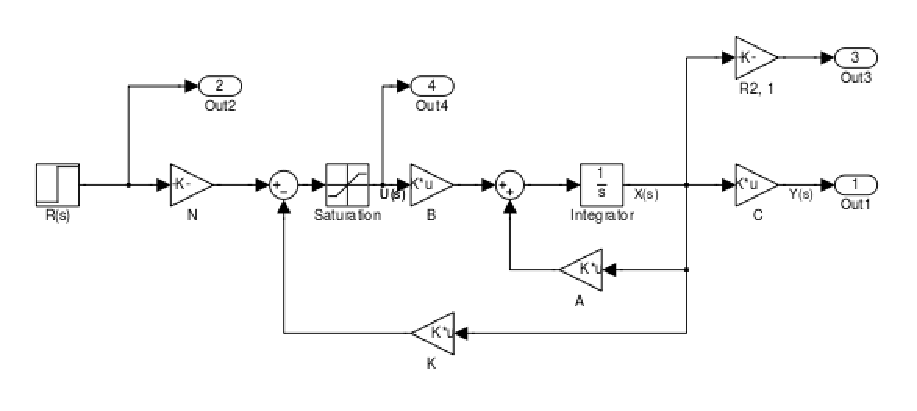
\includegraphics[width=350px]{full_state}
  \caption{Μοντέλο \textlatin{Simulink} συστήματος με ανάδραση κατάστασης.}
  \label{fig:full_state}
\end{figure}

Το μοντέλο \textlatin{Simulink} του συστήματος με ανάδραση κατάστασης υπάρχει στο αρχείο
\textlatin{\texttt{full\_ state.mdl}} και φαίνεται στο Σχήμα \ref{fig:full_state}.
Έχουμε να παρατηρήσουμε τα εξής σχετικά με το μοντέλο αυτό:
\begin{itemize}
	\item Η είσοδος αναφοράς ενισχύεται κατά παράγοντα Ν και στη συνέχεια τροφοδοτείται στο βρόχο του κλειστού συστήματος.
	      Το κέρδος Ν επιλέγεται έτσι ώστε το σφάλμα εξόδου μόνιμης κατάστασης για βηματική είσοδο να μηδενίζεται,
	      σύμφωνα με τη σχέση
	      \begin{equation}
	      	\label{eq:ref_gain}
	      	N = -\frac{\displaystyle 1}{\mathbf{C}(\mathbf{A}-\mathbf{B}\mathbf{D})^{-1} \mathbf{B}}
	      \end{equation}
	\item Σύμφωνα με την εκφώνηση η μέγιστη ροή εισόδου είναι $3 m^3/s$ και είναι θετική.
	      Για να εξασφαλισθεί ότι η ροή παραμένει πάντα μεταξύ των επιτρεπτών ορίων, έχει προστεθεί στο μοντέλο
	      ένα \textlatin{saturation block}.
\end{itemize}

Επιλέγοντας για τους επιθυμητούς πόλους απόσβεση $\zeta = 0.7$ ώστε να πληρούται η προδιαγραφή της μέγιστης υπερύψωσης
και κατάλληλο $ω_n$, παρατηρούμε από την προσομοίωση ότι το ύψος της μίας δεξαμενής ξεπερνά τα $6m$,
που σύμφωνα με της εκφώνηση είναι το μέγιστο ύψος των δεξαμενών.

Αυτό μας αναγκάζει να χρησιμοποιήσουμε μεγαλύτερο συντελεστή απόσβεσης.
Τελικά για $\zeta = 0.9$ και $ω_n = 0.0111 rad/s$ καλύπτονται ικανοποιητικά όλες τις προδιαγραφές.

Στα σχήματα \ref{fig:output_1} - \ref{fig:input_1} φαίνεται η χρονική απόκριση των διαφόρων μεταβλητών του συστήματος για
βηματική είσοδο αναφοράς $0.1 m^3/s$. Παρατηρούμε ότι η μέγιστη υπερύψωση της εξόδου είναι αμελητέα και
ο χρόνος αποκατάστασης είναι αρκετά κοντά στην προδιαγραφή των $400s$.

\section{Ελεγκτής με παρατηρητή πλήρους τάξης}
Σύμφωνα με την ιδιότητα του διαχωρισμού (\textlatin{\emph{separation property}}),
μπορούμε να χρησιμοποιήσουμε τα αποτελέσματα για τα κέρδη $\mathbf{K}$ και $N$ από την προηγούμενη ενότητα,
αλλά να αντικαταστήσουμε την ανάδραση πλήρους κατάστασης με έναν παρατηρητή πλήρους τάξης.

Οι δύο πόλοι του παρατηρητή επιλέχθηκε να έχουν $\zeta = 0.9$ (ίδιο με τους πόλους του κλειστού συστήματος)
και $ω_n = 0.0556 rad/s$ (πενταπλάσιο από τους πόλους του κλειστού συστήματος,
ώστε το σφάλμα του παρατηρητή να συγκλίνει αρκετά πιο γρήγορα από το σύστημα).

Και σε αυτή την περίπτωση χρησιμοποιούμε τον τύπο του \textlatin{Ackermann} για την εύρεση του
κέρδους $\mathbf{L}$ του παρατηρητή.

\begin{figure}[h]
  \centering
  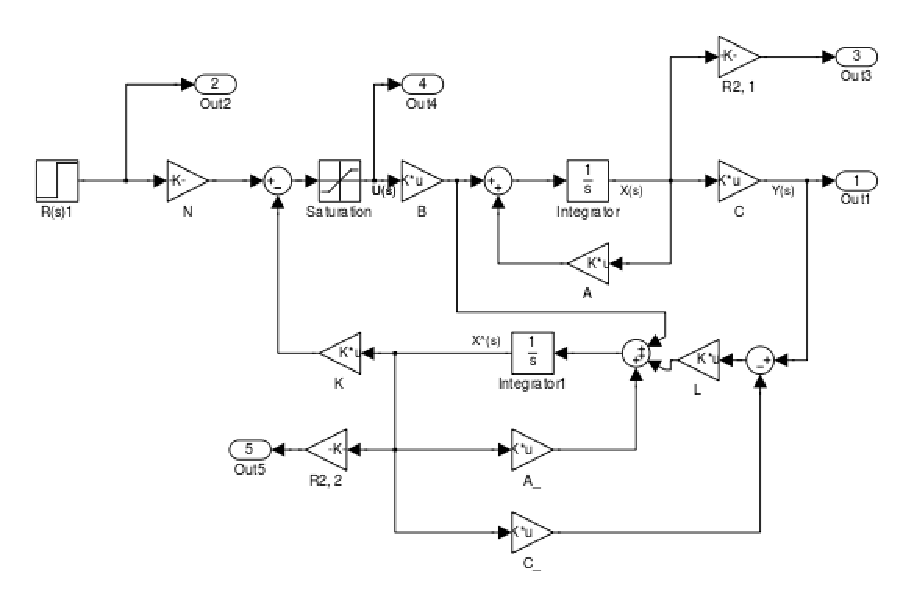
\includegraphics[width=350px]{full_obs}
  \caption{Μοντέλο \textlatin{Simulink} συστήματος με παρατηρητή πλήρους τάξης.}
  \label{fig:full_obs}
\end{figure}

Το μοντέλο \textlatin{Simulink} του κλειστού συστήματος με παρατηρητή πλήρους τάξης υπάρχει στο αρχείο
\textlatin{\texttt{full\_ obs.mdl}} και φαίνεται στο Σχήμα \ref{fig:full_obs}.
Στα σχήματα \ref{fig:output_2} - \ref{fig:input_2} φαίνεται η χρονική απόκριση των διαφόρων μεταβλητών του
συστήματος για βηματική είσοδο αναφοράς $0.1 m^3/s$.

Μπορούμε να παρατηρήσουμε ότι η απόκριση του συστήματος είναι σχεδόν πανομοιότυπη με το σύστημα ανάδρασης κατάστασης.
Αυτό οφείλεται αφ'ενός στο ότι ο παρατηρητής σχεδιάσθηκε έτσι ώστε να έχει αρκετά καλύτερα χαρακτηριστικά σύγλκισης
σε σχέση με το σύστημα και αφ'ετέρου επειδή δεν υπάρχουν πολύ απότομες μεταβολές στις καταστάσεις του συστήματος.
Κατά συνέπεια το σφάλμα παρατήρησης μηδενίζεται πολύ γρήγορα και το σύστημα συμπεριφέρεται σαν να είχαμε ανάδραση
πλήρους κατάστασης.

\section{Ελεγκτής με παρατηρητή μειωμένης τάξης}
Δεδομένου ότι η πρώτη μεταβλητή κατάστασης είναι η έξοδος του συστήματος ($x_1(t) = y(t) = q_0(t)$), μπορούμε
να την τροφοδοτούμε απ'ευθείας για ανάδραση και να σχεδιάσουμε έναν παρατηρητή πρώτης τάξης για την εκτίμηση
της δεύτερης μεταβλητής κατάστασης.

Σε αυτή την περίπτωση έχουμε να τοποθετήσουμε μόνο έναν πόλο και επιλέχθηκε να τοποθετηθεί στο
$-2\zeta ω_n$ για τις τιμές $\zeta$ και $ω_n$ που χρησιμοποιήθηκαν στον παρατηρητή πλήρους τάξης.

\begin{figure}[h]
  \centering
  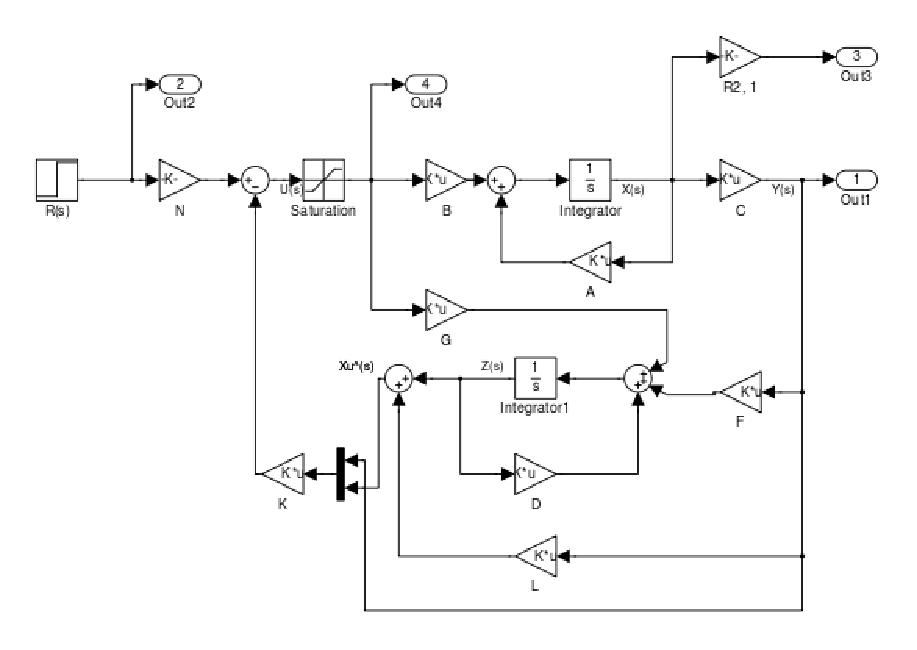
\includegraphics[width=350px]{reduced_obs}
  \caption{Μοντέλο \textlatin{Simulink} συστήματος με παρατηρητή μειωμένης τάξης.}
  \label{fig:reduced_obs}
\end{figure}

Το μοντέλο \textlatin{Simulink} του κλειστού συστήματος με παρατηρητή μειωμένης τάξης υπάρχει στο αρχείο
\textlatin{\texttt{reduced\_ obs.mdl}} και φαίνεται στο Σχήμα \ref{fig:reduced_obs}.
Στα σχήματα \ref{fig:output_3} - \ref{fig:input_3} φαίνεται η χρονική απόκριση των διαφόρων μεταβλητών του
συστήματος για βηματική είσοδο αναφοράς $0.1 m^3/s$.

Παρατηρούμε ότι και σε αυτή την περίπτωση τα αποτελέσματα είναι όμοια με τις προηγούμενες δύο.
Αυτό ήταν πλέον αναμενόμενο, δεδομένου ότι ούτως ή άλλως περιμέναμε ότι ο παρατηρητής μειωμένης τάξης
θα παρουσιάζει καλύτερη απόδοση από τον παρατηρητή πλήρους τάξης.

\begin{figure}[htb]
  \centering
  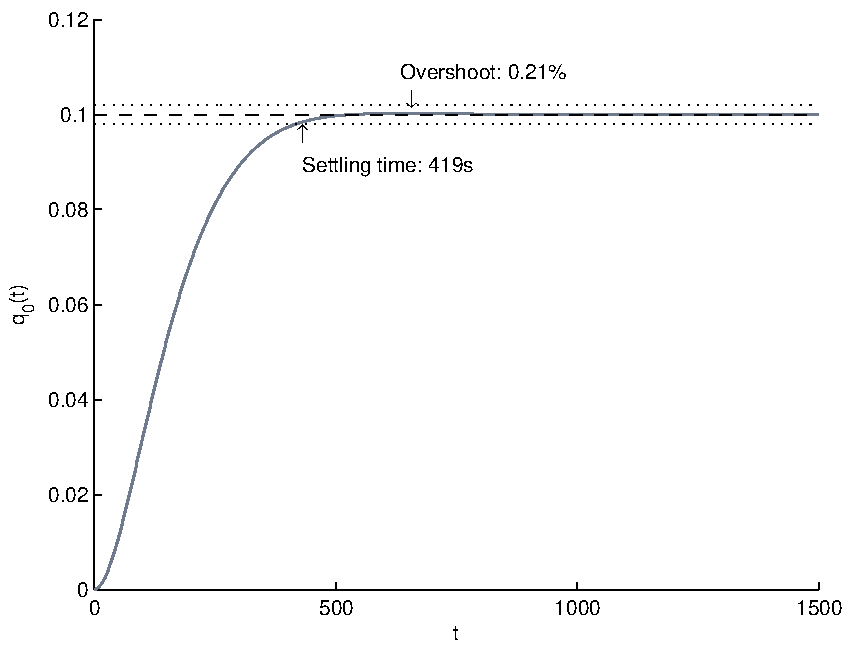
\includegraphics[width=300px]{output_1}
  \caption{Έξοδος συστήματος με ανάδραση κατάστασης.}
  \label{fig:output_1}
\end{figure}

\begin{figure}[htb]
  \centering
  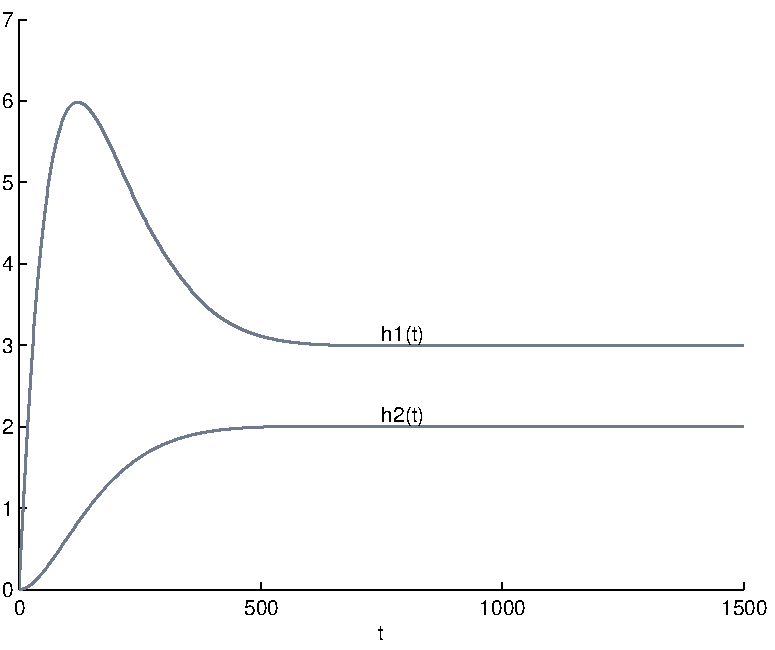
\includegraphics[width=300px]{heights_1}
  \caption{Ύψη δεξαμενών συστήματος με ανάδραση κατάστασης.}
  \label{fig:heights_1}
\end{figure}

\begin{figure}[htb]
  \centering
  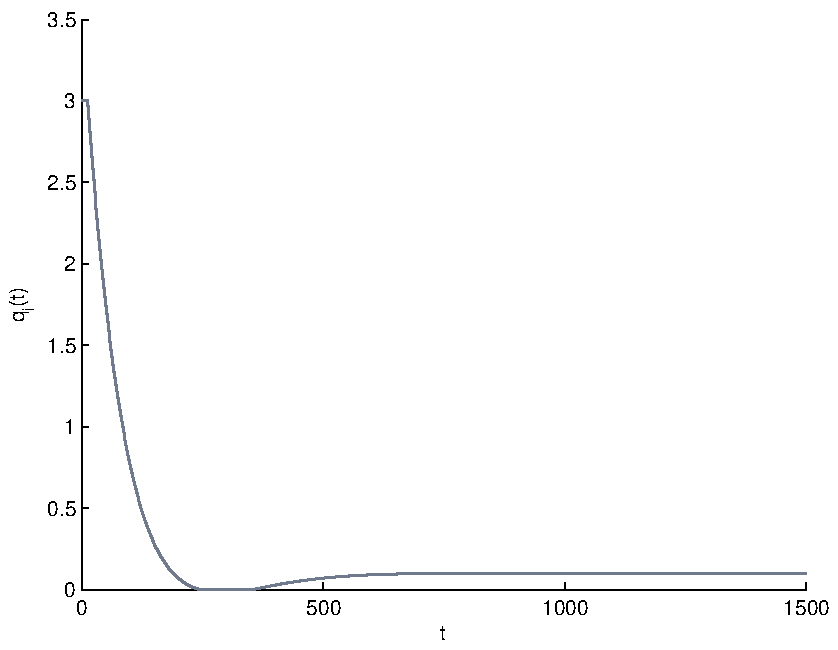
\includegraphics[width=300px]{input_1}
  \caption{Είσοδος ($q_i(t)$) συστήματος με ανάδραση κατάστασης.}
  \label{fig:input_1}
\end{figure}

\begin{figure}[htb]
  \centering
  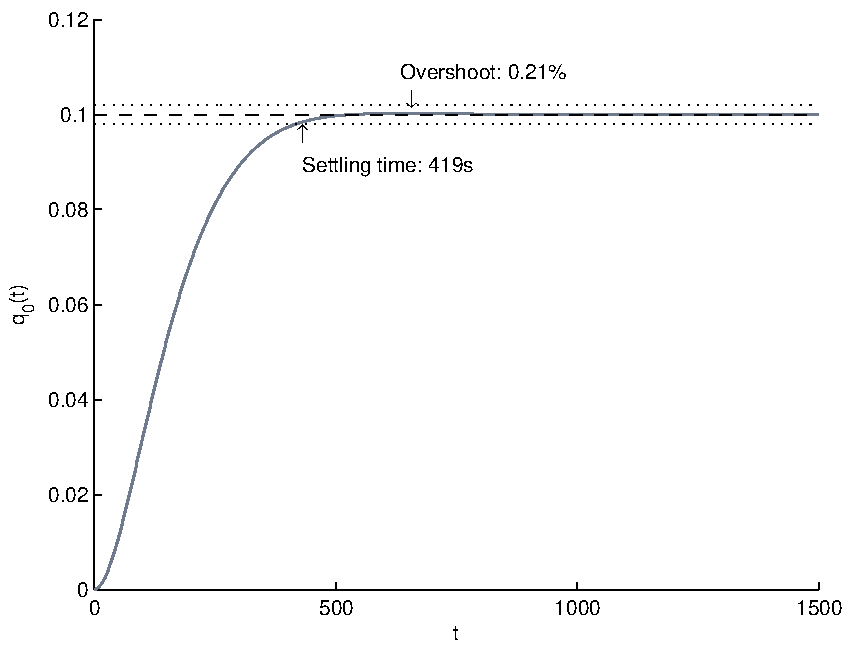
\includegraphics[width=300px]{output_2}
  \caption{Έξοδος συστήματος με παρατηρητή πλήρους τάξης.}
  \label{fig:output_2}
\end{figure}

\begin{figure}[htb]
  \centering
  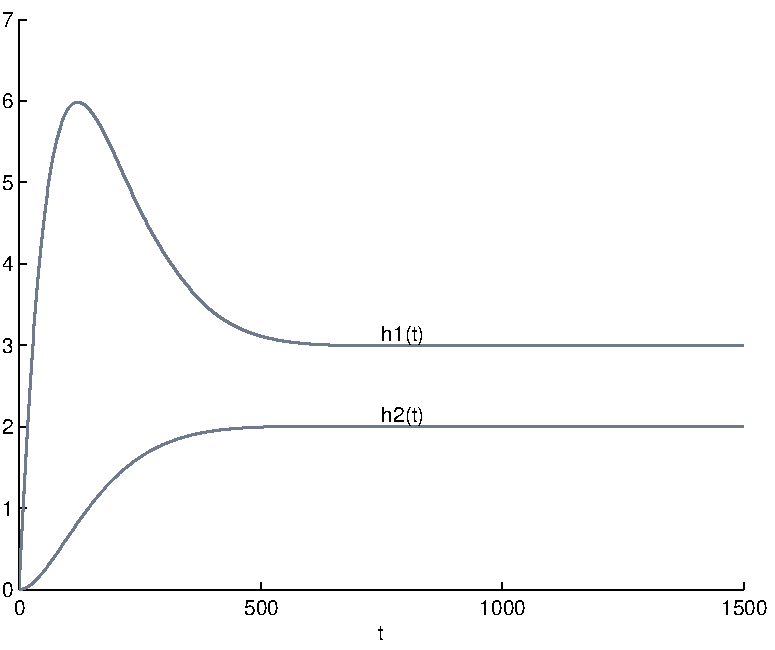
\includegraphics[width=300px]{heights_2}
  \caption{Ύψη δεξαμενών συστήματος με παρατηρητή πλήρους τάξης.}
  \label{fig:heights_2}
\end{figure}

\begin{figure}[htb]
  \centering
  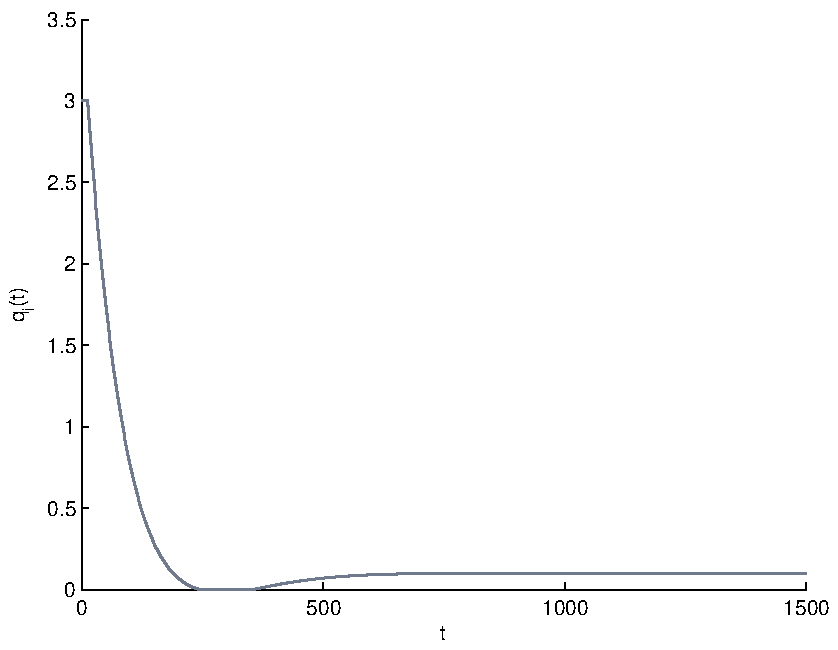
\includegraphics[width=300px]{input_2}
  \caption{Είσοδος ($q_i(t)$) συστήματος με παρατηρητή πλήρους τάξης.}
  \label{fig:input_2}
\end{figure}

\begin{figure}[htb]
  \centering
  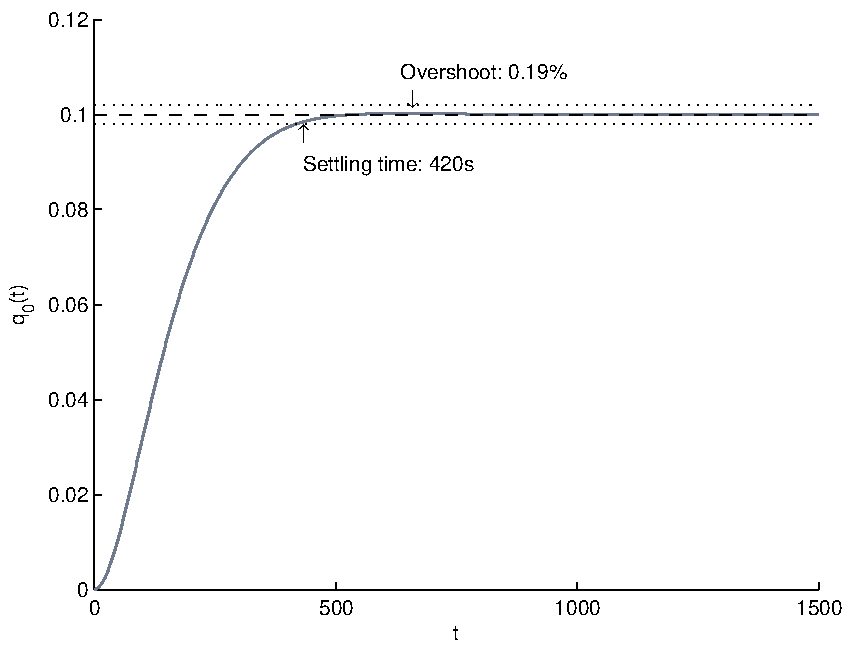
\includegraphics[width=300px]{output_3}
  \caption{Έξοδος συστήματος με παρατηρητή μειωμένης τάξης.}
  \label{fig:output_3}
\end{figure}

\begin{figure}[htb]
  \centering
  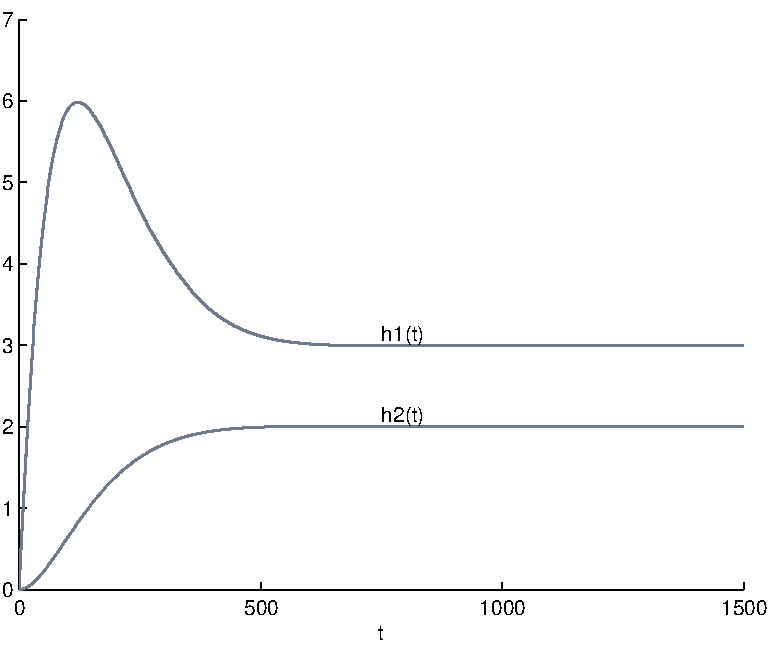
\includegraphics[width=300px]{heights_3}
  \caption{Ύψη δεξαμενών συστήματος με παρατηρητή μειωμένης τάξης.}
  \label{fig:heights_3}
\end{figure}

\begin{figure}[htb]
  \centering
  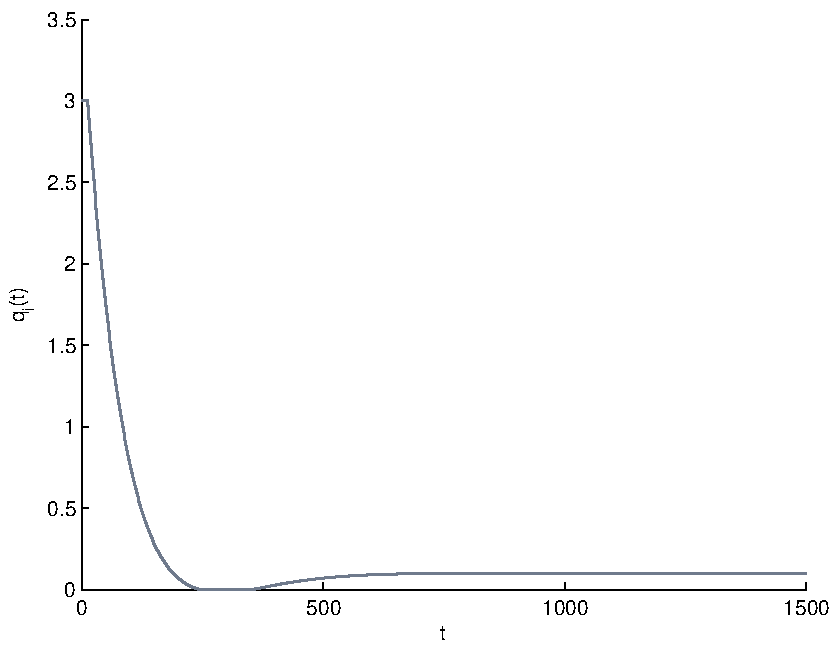
\includegraphics[width=300px]{input_3}
  \caption{Είσοδος ($q_i(t)$) συστήματος με παρατηρητή μειωμένης τάξης.}
  \label{fig:input_3}
\end{figure}

\end{document}